\todo[backgroundcolor=yellow]{SEC: Definition of a Network}
Community detection relies on us knowing lots about the underlying structure of a network and to do that we have to understand its properties. This chapter will establish a more formal understanding of networks and will highlight some key properties and methods that we will use to exctract value about community structure later.

\begin{definition}{(Undirected network)}
    Let $V$ be a set of vertices (nodes) and let $E$ be a set of pairs of vertices such that if $e = (x, y) \in E$ then $x, y \in V$. An undirected network is the pair $(V, E) = N$. An edge $e = (x, y) \in E$ is said to join $x$ and $y$ and $y$ to $x$.\cite[1]{oxford:renaud_notes}\label{def:undirected_network}
\end{definition}

The undirected network is the simplest type of network and on its own has interesting enough properties. However, for the sake of example and application, we will also introduce some other types of network that allow for more detailed models.

\todo[backgroundcolor=yellow]{SEC: Different Types of Network}

\begin{definition}{(Directed network)}
    Let $V$ be a set of vertices (nodes) and let $E$ be a set of pairs of vertices such that if $e = (x, y) \in E$ then $x, y \in V$. A directed network is the pair $(V, E) = N$. An edge $e = (x, y) \in E$ is said to join $x$ to $y$. I.e. if $x$ is joined to $y$ then $y$ is not necessarily joined to $x$.\cite[1]{oxford:renaud_notes}\label{def:directed_network}
\end{definition}

The intuition for directed graphs, is that edges may only be travelled along in one way. This comes in handy for modelling more intricate systems. The final network type of interest is that of the weighted network.

\begin{definition}{(Weighted network)}
    Let $V$ be a set of vertices (nodes) and let $E$ be a set of triples of the form $V^2 \times \mathbb{R}$ such that if $e = (x, y, w) \in E$ then $x, y \in V$. The value $w$ is said to be the weight of the edge.\cite[1]{oxford:renaud_notes}\label{def:weighted_network}
\end{definition}

The weighted network allows us to introduce some notion of how hard it is to move along a certain edge. This is useful when modeling things like traffic flow. [citation needed]

The above definitions of a network are likely more technical than we will ever need because once we have introduced the notion of of an adjacency matrix, that becomes our go to representation of a network.

\subsection{Adjacency Matrices}\todo[backgroundcolor=yellow]{SEC: Interesting Properties of Networks}
The objects defined above are meaningless without a rigorous way of mathematically representing them. To that end, we have to come up with a way of describing a network mathematically. This leads us to the definition of the adjacency matrix:

\begin{definition}{(Adjacency matrix)}
    Let $N = (V, E)$ be a network and label every vertex $v \in V$ with a number from $1$ to $n = |V|$. The adjacency matrix of a network is the matrix of elements $(A)_{ij}$ such that $a_{ij} = 1$ if $(i, j) \in E$ and $a_{ij} = 0$ if $(i, j) \notin E$. In other words, if nodes $i$ and $j$ are connected by an edge in the network, then the corresponding element in the matrix is $1$. Otherwise, it is $0$.\label{def:adjacency_matrix}\cite[111]{newman10}
\end{definition}

\begin{figure}
    \begin{center}
        \begin{subfigure}[b]{0.45\textwidth}
            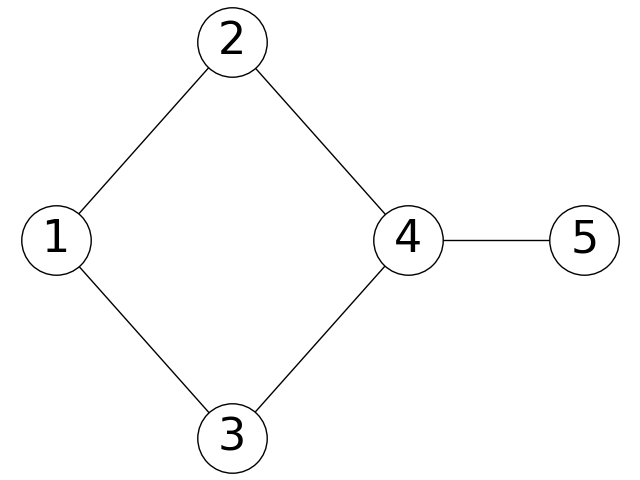
\includegraphics[width=\textwidth]{img/simple_example}
            \caption{Simple graph}
            \label{fig:simple_network}
        \end{subfigure}
        \begin{subfigure}[b]{0.45\textwidth}
            \begin{center}
            $
            \begin{pmatrix}
                0 & 1 & 1 & 0 & 0 \\
                1 & 0 & 0 & 1 & 0 \\
                1 & 0 & 0 & 1 & 0 \\
                0 & 1 & 1 & 0 & 1 \\
                0 & 0 & 0 & 1 & 0 \\
            \end{pmatrix}
            $
            \end{center}
            \caption{Adjacency matrix}
            \label{fig:simple_network_adjacency_matrix}
        \end{subfigure}
    \end{center}
    \caption{A simple network and its adjacency matrix}
    \label{fig:simple_network_and_adjacency_matrix}
\end{figure}

The adjacency matrix gives us our first way of representing a network. Figure \ref{fig:simple_network_and_adjacency_matrix} shows a basic example of a network and its associated adjacency matrix. This will form the basis for most of the analytical work we do going forwards. It's worth noting that there are also different types of adjacency matrix corresponding to the different types of network. For example, in the case of a directed network we will have a non-symmetric matrix where $a_{ij} = 1$ if $(i, j) \in E$ but this does not necessarily mean that $a_{ji} = 1$. We also get something similar for weighted networks where we set $a_{ij} = w$ where w is the weight of the edge connecting $i$ and $j$ in $N$.

\subsection{The Network Laplacian}
The Network Laplacian is a simple extension of the adjacency matrix with more interesting properties.

\begin{definition}{(Network Laplacian)}
    The Laplacian of a network $N = (V, E)$, denoted by $L$ is given by the following:
    $$ L = D - A $$
    where $A$ is the adjacency matrix of the network and $D$ is a diagonal matrix containing the degrees of each vertex in the network such that $d_{ii} = \text{deg}(v_i)$ and $d_{ij} = 0$ if $i \not= j$.
\end{definition}

\begin{figure}
    \begin{center}
        \begin{subfigure}[b]{0.45\textwidth}
            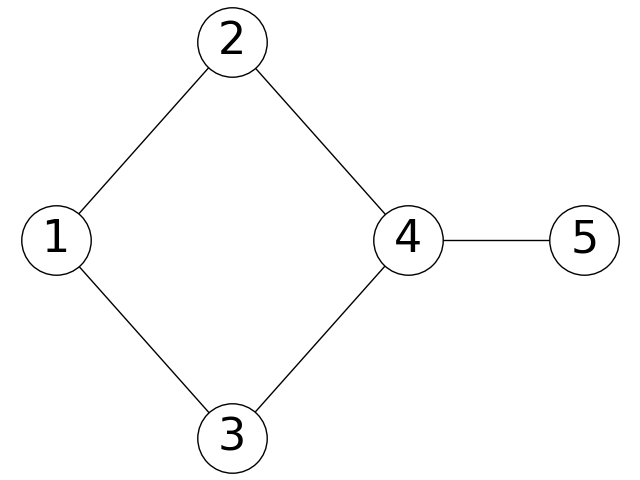
\includegraphics[width=\textwidth]{img/simple_example}
            \caption{Simple graph}
            \label{fig:simple_network_2}
        \end{subfigure}
        \begin{subfigure}[b]{0.45\textwidth}
            \begin{center}
            $
            \begin{pmatrix}
                 2 & -1 & -1 &  0 &  0 \\
                -1 &  2 &  0 & -1 &  0 \\
                -1 &  0 &  2 & -1 &  0 \\
                 0 & -1 & -1 &  2 & -1 \\
                 0 &  0 &  0 & -1 &  1 \\
            \end{pmatrix}
            $
            \end{center}
            \caption{Laplacian}
            \label{fig:simple_network_laplacian}
        \end{subfigure}
    \end{center}
    \caption{A simple network and its Laplacian}
    \label{fig:simple_network_and_laplacian}
\end{figure}

Figure \ref{fig:simple_network_and_laplacian} shows the same simple graph as before and it's Laplacian matrix.

\subsection{Paths}
When we're analysing a network, we're very often interested in which vertices are reachable from any given vertex. As such, we become interested in the idea of a path. A path in a network is defined in the following way

\begin{definition}{(Path)}
    Let $N = (V, E)$ be a network. A path is a sequence of vertices $v_1, \dots, v_n \in V$ such that $(v_i, v_{i+1}) \in E$ for all $i = 1, \dots, n-1$. In other words, a path is a sequence of vertices such that every consecutive pair of vertices is connected by an edge in $E$. We say that the length of a path is the number of edges $(v_i, v_{i+1})$ that are traversed by the path. Note that under this definition, we may pass through each vertex in the network more than once.
\end{definition}

Paths are an important concept in community detection as they allow us to phrase questions in rigorous terms as opposed to loose concepts of connectedness. Paths also give us our first look into the usefulness of the adjacency matrix. Using the adjacency matrix, it is very simple to determine whether there exists a path between two vertices $i$ and $j$. Paraphrasing Newman \cite[137]{newman10}, suppose our adjacency matrix is given by A. If $i$ and $j$ are directly connected then $A_{ij} = 1$ and we are done. If $A_{ij} = 0$ then pick some $k$ such that $A_{ik} = 1$. Then it is simple to see that if $A_{kj} = 1$ then $A_{ik}A_{kj} = 1$ which implies that $i$ and $j$ are connected via $k$. In fact, we can even go so far as to calculate the total number of ways to draw a path of length two between $i$ and $j$, $N^{(2)}_{ij}$, in the following way:

$$
N_{ij}^{(2)} = \sum_{k=1}^n A_{ik}A_{kj} = [A^2]_{ij}
$$

where $[\cdot]_{ij}$ denotes the $(i, j)$-th element of the given matrix. Clearly, this process actually generalises to paths of arbitrary length $r$ and we can see that

$$
N_{ij}^{(r)} = [A^r]_{ij}
$$

Also note that this solution counts each path but going in opposite directions. For example, you might have a path going $1 \rightarrow 4 \rightarrow 5 \rightarrow 2 \rightarrow 1$ which will also get counted separately by this method as the following $1 \rightarrow 2 \rightarrow 5 \rightarrow 4 \rightarrow 1$. This result isn't very useful, but it goes to show that the adjacency matrix we introduced before is useful and provides insight about the structure of our network. We call a path that starts and ends at the same place a loop and we can actually calculate the number of loops of length $r$ using the spectral properties of the adjacency matrix. Paraphrasing Newman again \cite[137]{newman10}, our adjacency matrix $A$ can be written as $A = UDU^T$ because $A$ is symmetric meaning that it has $n$ real and non-negative eigenvalues with real valued eigenvectors. In this form, $U$ is our matrix of eigenvectors and $D$ is the diagonal matrix containing the eigenvalues. We know that $A^r = (UKU^T)^r = UK^RU^T$ and then the number of loops is given by

$$
\begin{aligned}
    L_r &= \text{Tr}(UK^rU^T) = \text{Tr}(U^TUK^r) = \text{Tr}(K^r) \\
    & = \sum_i k_i^r
\end{aligned}
$$

where $k_i$ is the $i$-th entry of the matrix $K$. There exist analogous results for all the different types of networks which Newman discusses further. \cite[138]{newman10}. Typically, we are interested in types of path known as \emph{geodesic paths}.

\begin{definition}{(Geodesic Path)}
    A geodesic path (more commonly referred to as a shortest path) is a path through a network such that no shorter path exists.
\end{definition}

Geodesic paths are more interesting than general paths as they are necessarily self-avoiding as any time a path intersects with itself it adds unnecessary length. Geodesic paths are also used to define some other properties of networks such as the \emph{diameter}.

\subsection{Components}
Components are a natural consequence of the notion of paths. Simply put, components are sets of vertices in the graph that are all connected to each other via paths.

\begin{definition}{(Component)}
    A component is a subset $C$, of the vertex set $V$ such that if $v_1, v_2 \in C$ then $v_1$ and $v_2$ are connected by a path. Furthermore if $v_3 \not\in C$ then $v_3$ is not connected to either $v_1$ or $v_2$ by any path.
\end{definition}

Components are an important concept in the study of community detection. Recall the intuition for a community introduced in section \ref{sec:Introduction to Networks}. From here, it is clear to see a similarity between the notion of a community and that of a component. Loosely put, a community is a subset of a network that is \emph{nearly} a component.

\todo{This section probably need replacing with one on \emph{partitioning} and \emph{clustering}}

\subsection{Cut Sets}
Cut sets, as the name would suggest are sets of vertices that cut the network into multiple components. 

\begin{definition}{(Cut Set)}
    A cut set is a subset, $\mathcal{C}$, of the edge set, $E$, such that the network $N = (V, E\setminus\mathcal{C})$ has more than one component.
\end{definition}

We also have the notion of a minimum cut set which is a cut set of minimum cardinality. I.e. it's the smallest subset of the vertices that can be removed which will disconnect the network into two components. Similarly to components, minimum cut sets are also important in the analysis of communities as the size of the minimum cut gives us some notion of how strongly connected our network is. A larger cut set means that we require more edges to be removed from the network to get multiple connected components. This suggests that a network with a larger minimum cut is more strongly connected and a network with a smaller minimum cut is more loosely connected. An example of such structure can be seen in Figure \ref{fig:connectivity_strengths}.

\begin{figure}
    \begin{center}
        \begin{subfigure}[b]{0.45\textwidth}
            % 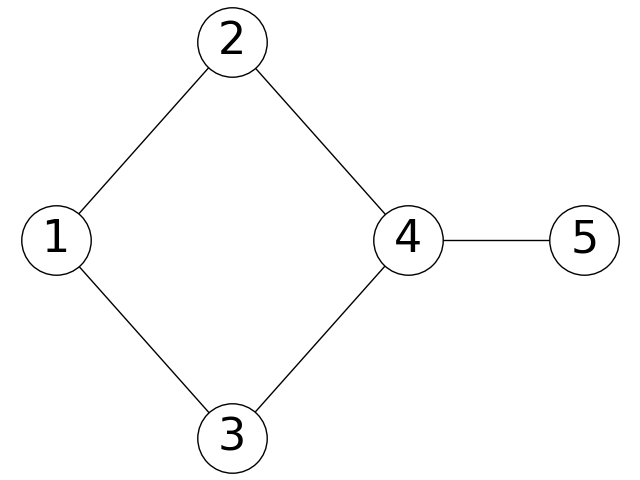
\includegraphics[width=\textwidth]{img/simple_example}
            \missingfigure{Strongly connected network}
            \caption{A strongly connected network}
            \label{fig:strongly_connected_network}
        \end{subfigure}
        \begin{subfigure}[b]{0.45\textwidth}
            \missingfigure{Loosely connected network}
            \caption{A loosely connected network}
            \label{fig:loosely_connected_network}
        \end{subfigure}
    \end{center}
    \caption{Two networks with differing connectedness}
    \label{fig:connectivity_strengths}
\end{figure}


\subsection{Degree Distribution}
We already know that the degree of a node is the number of edges incident on that node. In the context of adjacency matrices, the degree of node $i$ is defined by 

$$
\text{deg}(i) = d_i = \sum_{j=1}^NA_{ij}
$$

There also exist similar definitions for both weighted and directed networks. Using this definition of the degree of a matrix, we can define something called the \emph{degree distribution}. The degree distribution, as the name suggests, is a frequency distribution of all the degrees in the network. This distribution is often denoted by the function $p(k)$.

\begin{figure}
    \begin{center}
        \begin{subfigure}[b]{0.45\textwidth}
            % 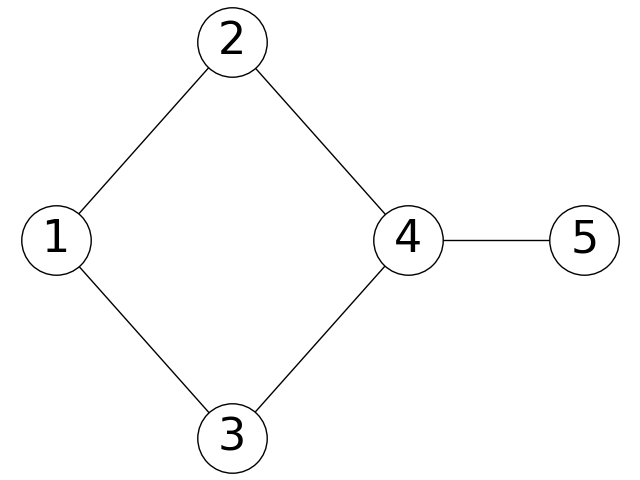
\includegraphics[width=\textwidth]{img/simple_example}
            \missingfigure{Zachary Karate Club}
            \caption{The Zachary Karate Club dataset}
            \label{fig:zachary_karate_club_degree}
        \end{subfigure}
        \begin{subfigure}[b]{0.45\textwidth}
            \missingfigure{Degree distribution of the Zachary Karate Club dataset}
            \caption{Degree Distribution of the Zachary Karate Club dataset}
            \label{fig:loosely_connected_network}
        \end{subfigure}
    \end{center}
    \caption{A network and it's associated degree distribution}
    \label{fig:connectivity_strengths}
\end{figure}

According to Renaud Lambiotte, these degree distributions often have very long tails which are regularly described by a power law. i.e.

$$ p(k) \propto k^{-\gamma} $$

where $\gamma$ usually takes values between $2$ and $3$.\cite[16]{oxford:renaud_notes} The relationship above holds approximately until some "cutoff degre" where the structure changes and $p(d)$ quickly decreases to $0$. Curiously, this leads us to a formalisation of the friendship paradox wherein the average number of friends of any given node is less than the average degree of nodes adjacent to any given node.

% \todo{in this section I'm finding it really hard not to just copy from Renaud's notes.}

% \subsection{Measures Derived from Walks and Paths}
% I think I'll probably leave this one out. It's not very interesting.

\subsection{Clustering Coefficient}
When thinking about community detection, we're actually interested in the connectedness of different parts of the network and in particular we're interested in the interconnectedness of a set of vertices. One way to measure the interconnectedness of a vertex with the surrounding nodes is using the clustering coefficient. The clustering coefficient counts the number of triangles in the network that include a given vertex. We define the clustering coefficient in the following way

$$ C_i = \frac{\text{number of triangles including the }i\text{th node}}{k_i(k_i-1)/2} $$

This quantity measures and normalises the number of triangles in the immediate vicinity of the vertex $i$. Using the clustering coefficient, we can extend this to consider the whole network.

$$ C = \frac{1}{N}\sum_{i=1}^NC_i $$

Again this total measure of clustering is normalised such that $0 \leq C \leq 1$.

% \subsection{Centrality}
% Different measures of centrality aim to convey the importance of certain nodes in the network. In this section, I will introduce some examples from Renaud Lambiotte's notes.\cite[19]{oxford:renaud_notes}
%
% \subsubsection{Closeness Centrality}
% The closeness centrality is the inverse of the mean distance between a node $i$ and every other node in the network. Notationally, this looks like the following
%
% $$ \text{closeness}_i = \frac{N - 1}{\sum_{j=1; j\not=i}^N d(i, j)} $$
%
% where $d(i, j)$ is the smallest number of moves from one node to another required to reach $j$ from $i$.
%
% \subsubsection{Betweenness Centrality}
% A slightly more complex measure of centrality is the betweenness centrality. This measures each node's contribution to the number of shortest paths that exist in the network.
%
% $$ \text{betweenness}_i = \frac{2}{(N-1)(N-2)}\sum_{j=1; j\not=i}^N \sum_{l=1; l\not=i}^{j-1} \frac{\sigma_{jl}^i}{\sigma_{jl}}, $$
%
% where $\sigma_{jl}$ denotes the total number of shortest paths connecting nodes $j$ and $l$ and $\sigma_{jl}^i$ is the number of such paths containing the node $i$.
%
% \subsubsection{Katz Centrality}
% The Katz measure of centrality considers all walks between two nodes $i$ and $j$, but gives each one less weighting as it increases in length by scaling it by a constant $\alpha \in (0, 1)$. The Katz centrality of a node $i$ is defined by
%
% $$ \text{Katz}_j = \sum_{i=1}^N[(I - \alpha A)^{-1}]_{ij}. $$
%
% \subsubsection{PageRank}
% PageRank is a centrality measure developed with the advent of the internet in an attempt to improve search engine indexing.\cite{pagerank} The actual algorithm for PageRank is too intricate to go into here, but the intuition fir it is that ``highly linked pages are more important than pages with few links"\cite[3]{pagerank}
%
\subsection{Centrality}
The core idea of centrality is to formalise the importance of certain nodes in the network. There are, of course, a number of ways to do this. Lambiotte covers a number of centrality measures \cite[18]{oxford:renaud_notes} which are reprinted here in order of increasing complexity. To begin, we shall talk about closeness centrality. Simply put, the closeness centrality is the inverse of the mean distance between a node $i$ and every other node in the network. Notationally, this looks like the following:

$$ \text{closeness}_i = \frac{N - 1}{\sum_{j=1; j\not=i}^N d(i, j)}, $$

where $d(i, j)$ is the smallest number of edges that must be traversed to reach $j$ from $i$. As an initial measure of centrality, this holds up well. It clearly meets the criterion of identifying nodes that are important in the network as nodes that are close to most other nodes have a very high closeness centrality whilst nodes that exist on the peripherals of a network have a low closeness centrality.

However, this measure doesn't consider the importance of nodes when traversing the network. Betweeness centrality looks to solve this problem by counting the each node's contribution to the number of shortest paths that exist in the network. Betweeness centrality is calculated in the following way:

$$ \text{betweenness}_i = \frac{2}{(N-1)(N-2)}\sum_{j=1; j\not=i}^N \sum_{l=1; l\not=i}^{j-1} \frac{\sigma_{jl}^i}{\sigma_{jl}}, $$

where $\sigma_{jl}$ denotes the total number of shortest paths connecting nodes $j$ and $l$ and $\sigma^i_{jl}$ is the number of such paths containing the node $i$. This measure clearly fixes the issue that closeness centrality had by considering how many paths use a given node $i$, but what if a node rarely contributes to shortest paths, but often contributes to near-shortest paths? We would expect a good measure of the importance of a node in a network to use at least some contribution from near shortest paths. Katz centrality does this by considering all paths connecting a node to every other node and giving longer paths less weight. Katz centrality is calculated as follows:

$$ \text{Katz}_j = \sum_{i=1}^N[(I - \alpha A)^{-1}]_{ij}, $$

where $\alpha \in (0, 1)$ is an absolute constant. These methods all build up to more complicated measures such as PageRank\cite{pagerank} which solves exactly the same problem, but using more advanced and intricate techniques and not necessarily on undirected networks.

\subsection{Spectral Properties}
The final properties of interest are spectral in nature. Spectral properties are properties that are based on the eigendecomposition of either the adjacency matrix, the Laplacian or a modified version of the Laplacian called the normalised Laplacian. If the Laplacian is defined by
$$ L = D - A, $$
Then the normalised Laplacian is given by 
$$ \tilde L = D^{-1/2}LD^{-1/2} = I - D^{-1/2}AD^{-1/2}. $$

By definition, the adjacency matrix, the Laplacian and the normalised Laplacian are symmetric. This means that the eigenvalues of each matrix are all real and the corresponding eigenvectors form an orthonormal basis. It's important to note that the two Laplacian matrices always have $\lambda_1 = 0$. In fact, if the network is connected, $\lambda_1 = 0$ and $\lambda_i > 0 \; \forall i > 1$. This is our first spectral property of a matrix. More advanced spectral properties are used to solve community detection problems such as finding a minimum cut (see section \ref{sec:smallest_cut}). Introduction of spectral ideas concludes this section on properties of interest. Now that all of the necessary vocabulary and concepts are introduced, we are ready to discuss community detection.
